%% This is file `IPPbeamer.tex' version 2.2 (2022/07/23),
%% it is part of the IPP-bundle
%% Beamer-slides and tcolorbox-posters for IPP
%% ----------------------------------------------------------------------------
%%
%%  Copyright (C) 2020–2023 by Marei Peischl <marei@peitex.de>
%%
%% ============================================================================
%% This work may be distributed and/or modified under the
%% conditions of the LaTeX Project Public License, either version 1.3c
%% of this license or (at your option) any later version.
%% The latest version of this license is in
%% http://www.latex-project.org/lppl.txt
%% and version 1.3c or later is part of all distributions of LaTeX
%% version 2008/05/04 or later.
%%
%% This work has the LPPL maintenance status `maintained'.
%%
%% Thecurrent maintainer of this work is
%%   Marei Peischl <marei@peitex.de>
%%
%% ============================================================================
%%
\documentclass[
	english,% main language as global option
	logo=false,% logo to be used in the headline. Pre-defined values are: asdex, w7x, false. Initial value is empty
	eurofusion=false, %initial value is false
	titlegraphic=true, %initial value is false
	]{ippbeamer}

\usepackage{amsmath}
\usepackage{amsfonts}
\usepackage{amssymb}
\usepackage{amsthm}
\usepackage{bm}
\usepackage{caption}
\usepackage{xcolor}
\usepackage{csquotes}
\usepackage{enumerate}
\usepackage{faktor}
\usepackage{graphicx}
\usepackage{hyperref}
\usepackage{listings}
\usepackage{mathrsfs}
\usepackage{mathtools}
\usepackage{pgf,tikz}
\usepackage{pgfplots, pgfplotstable}
% \usepackage{showlabels}
\usepackage{svg}
\usepackage{tikz-cd}
\usepackage{url}

\usepackage{subcaption} 

\pgfplotsset{compat=1.18}
\usetikzlibrary{arrows}
\usetikzlibrary{decorations.pathreplacing,decorations.markings}

\definecolor{codegreen}{rgb}{0,0.6,0}
\definecolor{codegray}{rgb}{0.5,0.5,0.5}
\definecolor{codepurple}{rgb}{0.58,0,0.82}
\definecolor{backcolour}{rgb}{0.95,0.95,0.92}


\lstdefinestyle{mystyle}{
    backgroundcolor=\color{backcolour},   
    commentstyle=\color{codegreen},
    keywordstyle=\color{magenta},
    numberstyle=\tiny\color{codegray},
    stringstyle=\color{codepurple},
    basicstyle=\ttfamily\footnotesize,
    breakatwhitespace=false,         
    breaklines=true,                 
    captionpos=b,                    
    keepspaces=true,                 
    % numbers=left,                    
    numbersep=5pt,                  
    showspaces=false,                
    showstringspaces=false,
    showtabs=false,                  
    tabsize=2
}

\lstset{style=mystyle}

\captionsetup[figure]{labelformat=empty}

% \newtheorem{lemma}{Lemma}[section]
% \numberwithin{lemma}{section}
% \newtheorem{corollary}[lemma]{Corollary}
% \newtheorem{proposition}[lemma]{Proposition}
% \newtheorem{theorem}[lemma]{Theorem}

% \theoremstyle{definition}
% \newtheorem{assumption}[lemma]{Assumption}
% \newtheorem{definition}[lemma]{Definition}
% \newtheorem{example}[lemma]{Example}
% \newtheorem{remark}[lemma]{Remark}
% \newtheorem{problem}[lemma]{Problem}

\DeclareMathOperator{\grad}{grad}
\DeclareMathOperator{\curl}{curl}
\DeclareMathOperator{\diver}{div}

\newtheorem{assumption}{Assumption}




% some adjustments which are generally not available
\let\code\texttt
\let\file\texttt

% extended graphicspath to use separate image directories without the bundle being installed
\graphicspath{{}{img/}{img/titlegraphic/}}

\title{Requirements for multipatch geometry}
% \subtitle{presentations using \LaTeX}
\author{Pauline Vidal, Alexander Hoffmann}
% \institute{\inst{1}pei\TeX{} \and\inst{2}Institut 2}
\date{\today}
% Additional Logo to be placed in the footer
% \logo{\includegraphics[height=\height]{example-image}}

\begin{document}


\frame{\titlepage}

\begin{frame}{Questions to be answered}
	\vspace*{1cm}
	\begin{exampleblock}{}
		What is the most suited way to solve the problems related to multipatch
		in our case?
	\end{exampleblock}
	\vspace*{0.5cm}
	\begin{exampleblock}{}
		What could be missing in the DDC library to implement multipatch?
	\end{exampleblock}
\end{frame}


\begin{frame}{Structure of multi-patch}

\begin{figure}[!h]
\begin{subfigure}{0.8\textwidth}
\centering
\tiny
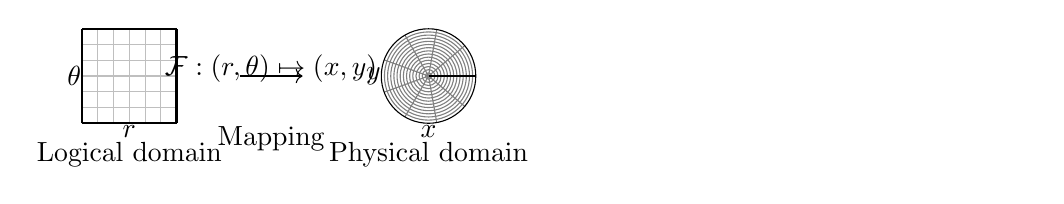
\begin{tikzpicture}[xscale = 0.4, yscale = 0.4]
	% logical grid
	\draw[lightgray] (0,0) grid [step = 0.5] (3,3);
	\draw[thick] (0,0) grid [step = 3] (3,3);
	
	\node at (-0.25, 1.5) {$\theta$}; 
	\node at (1.5, -0.25) {$r$}; 
	
	\node at (1.5,-1) {Logical domain} ; % subtitle
	
	% mapping
	\begin{scope}[xshift =1.5cm]	
		\draw[->] (3.5, 1.5) -- (5.5, 1.5); 
		\node at (4.5,1.75) {$\mathcal{F}:(r,\theta)\mapsto(x,y)$}; 
		
		\node at (4.5,-0.5) {Mapping} ; % title
	\end{scope}
	
	\begin{scope}[xshift = 11cm, yshift = 1.5cm]	
		% physical grid
		\def\Rmax{1.5}
		\foreach \r in {0, 0.1, ...,\Rmax} {
		    \draw[gray] (0,0) circle (\r);
		}
		\foreach \theta in {0, 40,...,360} {
    			\draw[gray] (0,0) -- (\theta:\Rmax);
		}
		
		\draw[black] (0,0) circle (\Rmax);
		\draw[black] (0,0) -- (0:\Rmax);
		
		\node at (-1.75, 0) {$y$}; 
		\node at (0, -1.75) {$x$}; 
		
		\node at (0,-2.5) {Physical domain} ; % subtitle
	\end{scope}
	
	\node at (30,0) { }; % just to put the figure on the left side on the slide. 
	
	
	
\end{tikzpicture}
\end{subfigure}
\begin{subfigure}{0.2\textwidth}
\centering
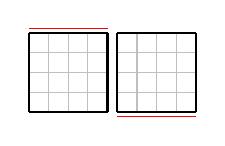
\begin{tikzpicture}[xscale = 0.5, yscale = 0.5]
	\draw[lightgray] (0,0) grid [step = 0.5] (2,2);
	\draw[thick] (0,0) grid [step = 2] (2,2);
	
	\draw[red] (0,2.125) -- (2,2.125);
	
	\begin{scope}[shift={(2.25,0)}]
		\draw[lightgray] (0,0) grid [step = 0.5] (2,2);
		\draw[thick] (0,0) grid [step = 2] (2,2);
		
		\draw[red] (0,-0.125) -- (2,-0.125);
	\end{scope}
\end{tikzpicture}
\caption{\scriptsize Simple interface.}
\end{subfigure}
\begin{subfigure}{0.2\textwidth}
\centering
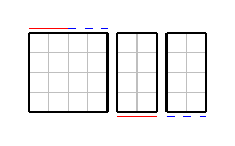
\begin{tikzpicture}[xscale = 0.5, yscale = 0.5]
	\draw[lightgray] (0,0) grid [step = 0.5] (2,2);
	\draw[thick] (0,0) grid [step = 2] (2,2);
	
	\draw[red] (0,2.125) -- (1,2.125);
	\draw[blue, dashed] (1,2.125) -- (2,2.125);
	
	\begin{scope}[shift={(2.25,0)}]
		\draw[lightgray] (0,0) grid [step = 0.5] (1,2);
		\draw[thick] (0,0) grid [xstep = 1, ystep=2] (1,2);
		\draw[red] (0,-0.125) -- (1,-0.125);
	\end{scope}
	
	\begin{scope}[shift={(3.5,0)}]
		\draw[lightgray] (0,0) grid [step = 0.5] (1,2);
		\draw[thick] (0,0) grid [xstep = 1, ystep=2] (1,2);
		\draw[blue, dashed] (0,-0.125) -- (1,-0.125);
	\end{scope}
	
\end{tikzpicture} 
\caption{\scriptsize T-joint. }
\end{subfigure}
\begin{subfigure}{0.4\textwidth}
\centering
\tiny
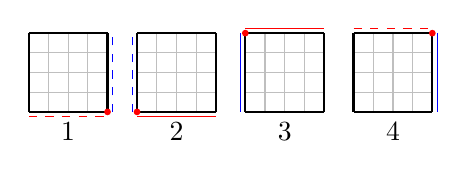
\begin{tikzpicture}[xscale = 0.5, yscale = 0.5]
	% grid
	\foreach \x in {0, ..., 3}{
		\begin{scope}[shift={(2.75*\x,0)}]
			\draw[lightgray] (0,0) grid [step = 0.5] (2,2);
			\draw[thick] (0,0) grid [step = 2] (2,2);
		\end{scope}
	}
	
	\node at (1,-0.5) {1};
	\node at (1+2.75,-0.5) {2};
	\node at (1+2.75*2,-0.5) {3};
	\node at (1+2.75*3,-0.5) {4};
	
	% Xpoint
	\draw[fill = red, color=red]  (2,0) circle (2pt);
	\draw[fill = red, color=red]  (2.75,0) circle (2pt);
	\draw[fill = red, color=red]  (2.75*2,2) circle (2pt);
	\draw[fill = red, color=red]  (2+2.75*3,2) circle (2pt);
	
	% Interfaces
	\draw[red] (0+2.75,-0.125) -- (2+2.75,-0.125);
	\draw[red] (0+2.75*2,2.125) -- (2+2.75*2,2.125);
	
	\draw[red, dashed] (0,-0.125) -- (2,-0.125);
	\draw[red, dashed] (0+2.75*3,2.125) -- (2+2.75*3,2.125);
	
	\draw[blue] (-0.125+2.75*2,0) -- (-0.125+2.75*2,2);
	\draw[blue] (2.125+2.75*3,0) -- (2.125+2.75*3,2);
	
	\draw[blue, dashed] (2.125,0) -- (2.125,2);
	\draw[blue, dashed] (-0.125+2.75,0) -- (-0.125+2.75,2);
	
	
\end{tikzpicture}
%\caption{X-point in logical domain.}
%\end{subfigure}
%\begin{subfigure}{0.2\textwidth}
	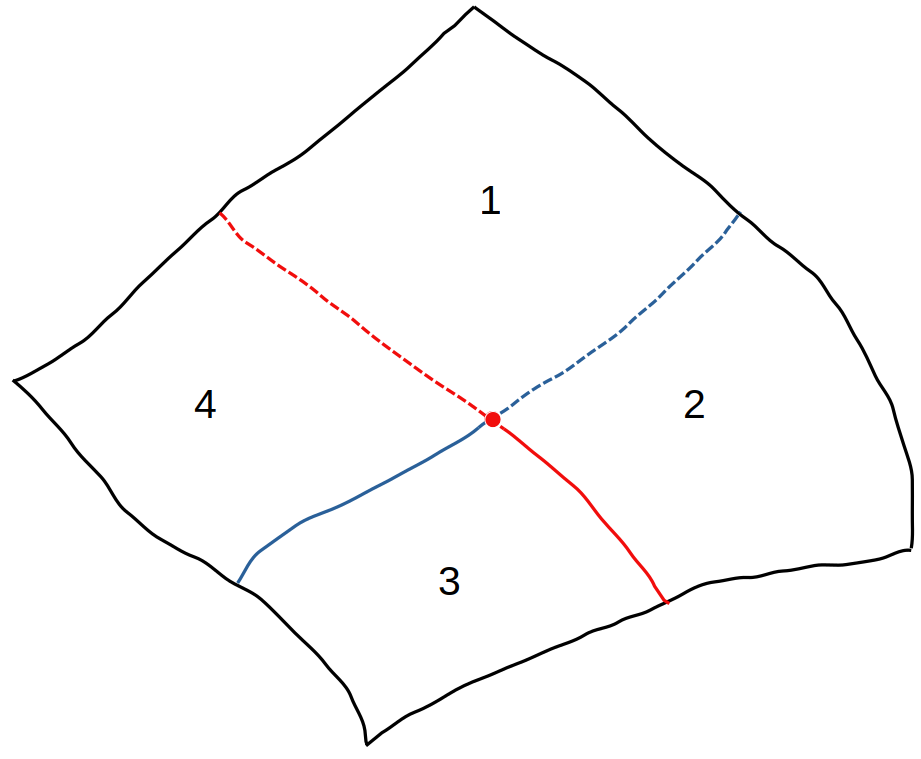
\includegraphics[width=3cm]{../images/X_point_in_physical.png}
\caption{\scriptsize X-point in logical and physical domain.}
\end{subfigure}
\caption{\footnotesize \label{Patches_logical_dom} Patches in the logical domain.}
\end{figure}


\end{frame}


\begin{frame}{Advection}
\footnotesize
\begin{equation}
\begin{aligned}
	\partial_t \rho + A\cdot\nabla \rho = 0,
	\qquad \qquad
	\partial_t X(t^{n}; t^{n+1}, x)  = A(t, X(t^{n}; t^{n+1}, x)).
\end{aligned}
\label{guiding_center_eq}
\end{equation}

\begin{figure}[!h]
\centering
\tiny
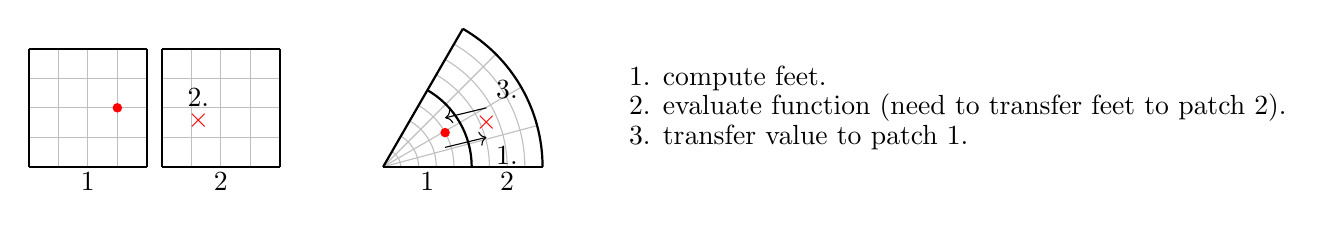
\begin{tikzpicture}[xscale = 0.75, yscale = 0.75]
	% logical grid 
	\draw[lightgray] (0,0) grid [step = 0.5] (2,2);
	\draw[thick] (0,0) grid [step = 2] (2,2);
	\node at (1, -0.25) {$1$};
	
	\begin{scope}[xshift=2.25cm]
		\draw[lightgray] (0,0) grid [step = 0.5] (2,2);
		\draw[thick] (0,0) grid [step = 2] (2,2);
		\node at (1, -0.25) {$2$};
	\end{scope}
	
	% feet
	\draw[fill = red, color=red]  (1.5,1) circle (2pt);
	\node at (2.87, 0.78) {\color{red} $\times$};
	
	\node at (2.87, 0.78+0.4) {2.};
	
	\begin{scope}[xshift=6cm]
		% physical grid
		\def\RmaxA{1.5}
		\def\RmaxB{2.7}
		\foreach \r in {0, 0.3, ...,\RmaxB} {
		    \draw[lightgray] (0,0) ++(0:\r) arc (0:60:\r);
		}
		\foreach \theta in {0, 15, ..., 60} {
    			\draw[lightgray] (0,0) -- (\theta:\RmaxB);
		}
		\node at (0.75, -0.25) {$1$};
		\node at (2.1, -0.25) {$2$};


		\draw[thick, black] (0,0) ++(0:\RmaxA) arc (0:60:\RmaxA);
		\draw[thick, black] (0,0) ++(0:\RmaxB) arc (0:60:\RmaxB);
		
		\draw[thick, black] (0,0) -- (0:\RmaxB);
		\draw[thick, black] (0,0) -- (60:\RmaxB);
		
		% feet
		\draw[fill = red, color=red]  (1.05,0.58) circle (2pt);
		\node at (1.75, 0.75) {\color{red} $\times$};
		
		\draw[->] (1.05, 0.58-0.25) -- (1.75, 0.75-0.25) node[below right]{1.}; 
		\draw[<-] (1.05, 0.58+0.25) -- (1.75, 0.75+0.25) node[above right]{3.}; 
	\end{scope}
	
	% legend
	\begin{scope}[xshift=10cm]	
		\node[right] at (0,1.5) {1. compute feet.};
		\node[right] at (0,1) {2. evaluate function (need to  transfer feet to patch 2).};
		\node[right] at (0,0.5) {3. transfer value to patch 1.};
	\end{scope}
\end{tikzpicture}
\caption{\scriptsize Example of a characteristic foot outside the patch 1 in the logical and physical domains.}
\end{figure}


\begin{figure}
\centering
\tiny
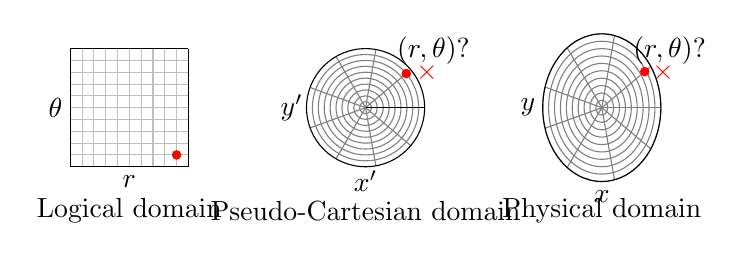
\begin{tikzpicture}[xscale = 0.75, yscale = 0.75]
	% logical domain
	\draw[lightgray] (0,0) grid [step = 0.2] (2,2);
	\draw[black] (0,0) grid [step = 2] (2,2);
	
	\node at (-0.25, 1) {$\theta$}; 
	\node at (1, -0.25) {$r$}; 
	\node at (1,-0.75) {Logical domain} ;
	
	\draw[fill = red, color=red]  (1.8,0.2) circle (2pt);
	
	% pseudo Cartesian domain
	\begin{scope}[xshift=5cm, yshift = 1cm]
		\def\Rmax{1}
		\foreach \r in {0, 0.1, ...,\Rmax} {
		    \draw[gray] (0,0) circle (\r);
		}
		\foreach \theta in {0, 40,...,360} {
    			\draw[gray] (0,0) -- (\theta:\Rmax);
		}
		
		\draw[black] (0,0) circle (\Rmax);
		\draw[black] (0,0) -- (0:\Rmax);
		
		\node at (-1.25, 0) {$y'$}; 
		\node at (0, -1.25) {$x'$}; 
		\node at (0,-1.75) {Pseudo-Cartesian domain} ; % subtitle
		
		\draw[fill = red, color=red]  (40:\Rmax-0.1) circle (2pt);
		\node at (30:\Rmax+0.2) {\color{red} $\times$};
		\node at (40:\Rmax+0.5) {$(r,\theta)$?};
	\end{scope}
	
	
	% physical domain
	\begin{scope}[xshift=9cm, yshift = 1cm]
		\def\Rmax{1} 
		\def\numTheta{10} 
		\def\a{1} 
		\def\b{1.25} 
		
		\foreach \r in {0,0.1,...,\Rmax} {
		    \draw[gray] (0,0) ellipse ({\a-\r*(\a/\Rmax)} and {\b-\r*(\b/\Rmax)});
		}
		
		\foreach \theta in {0,40,...,360} {
			\def\radius{\a*\b / sqrt(\b*\b*cos(\theta)*cos(\theta) + \a*\a*sin(\theta)*sin(\theta))} 
		    \draw[gray] (0,0) -- (\theta:{\radius});
		}
		
		\draw[black] (0,0) ellipse ({\a} and {\b});
		
		\node at (-1.25, 0) {$y$}; 
		\node at (0, -1.5) {$x$}; 
		\node at (0,-1.75) {Physical domain} ;
		
		\draw[fill = red, color=red]  (40:\Rmax-0.05) circle (2pt);
		\node at (30:\Rmax+0.2) {\color{red} $\times$};
		\node at (40:\Rmax+0.5) {$(r,\theta)$?};
	\end{scope}
	
	
\end{tikzpicture}
\end{figure}
\end{frame}

\begin{frame}{Solving Poisson with CONGA}
	We want to solve the Poisson equation
	\begin{align*}
		-\diver (\nu \grad \phi) = \rho
	\end{align*}
	using a the CONGA approach on a 2D multipatch domain. 
	\begin{itemize}
		\item Have finite element space $V_h$ with jump discontinuities across edges
		\item Subspace $V_h^c \subseteq V_h$ with functions conforming to some global
				regularity constraint
		\item Define projection $P_h: V_h \rightarrow V_h^c$
				and discrete differential operator $\grad_h \vcentcolon= \grad P_h$
				$\rightarrow$ need information on mesh and spline degree of neighboring patches
		\item Discretize Poisson equation weakly using these operators
	\end{itemize}
\end{frame}

\begin{frame}{Solving Poisson with CONGA}
	\vspace*{1.5cm}
	\begin{alertblock}{\textbf{Advantages}}
		\begin{itemize}
			\item Already implemented in Psydac and successfully applied to several problems. 
			\item Probably easier to generalize to complicated geometries than other approaches
					like using different splines e.g.
		\end{itemize}
	\end{alertblock}
\end{frame}



\begin{frame}{Patch data -- Exchange}
	\begin{itemize}
		\item Mesh-points,
		\item Local sums to compute the derivatives at the interfaces
				\begin{align*}
					\sum_{x_i \in \text{global space}} \alpha_i s(x_i) = \sum_{p \in\text{Patches}} 
							\sum_{x_i \in p} \alpha_i s(x_i),
				\end{align*}
		where $\alpha_i$ depend on the mesh points,
		\item Characteristic feet outside of the patch,
		\item Interpolated values for $\mathbf{A}$ and $\rho$.
	\end{itemize}
\end{frame}
\begin{frame}{Patch data -- Storage}
	\begin{itemize}
		\item Mesh points, dimension (\texttt{DimXi}, \texttt{DimYi}), mapping,
				\texttt{SplineBuilder}, metadata, 
		\item Boundary condition of global domain if an edge of the patch is on the global boundary,
		\item Values of functions $\rho$, $\phi$, $\mathbf{A}$ on mesh points,
		\item Spline coefficients of functions ($\rho$, $\phi$, $\mathbf{A}$),
		\item Reference to global domain class.
	\end{itemize}
\end{frame}

\begin{frame}{Global domain}
	\begin{itemize}
		\item Global domain class
		\begin{itemize}
			\item References to patches,
			\item 'Connectivity' class which encodes the geometrical information.
		\end{itemize}
		\item Connectivity class
		\begin{itemize}
			\item Identify edges and corners of different patches
			\item For T-joint, identify sections of edges with sections of other edges, 
					place corners in the middle of edges.
		\end{itemize}
		
	\end{itemize}
	\end{frame}


\begin{frame}{APPENDIX - Structure code}
\vspace*{0.5cm}
\centering
\scriptsize

\begin{columns}
\begin{column}{0.5\textwidth}
\begin{tabular}{|l|}
	\hline
	\textbf{\textsc{Global domain class}} \\
	\hline
	\textit{Define a global view of the domain.} \\
	$\bullet$ Reference to each Patch object.\\
	$\bullet$ Global boundaries (outside boundaries).\\
	$\bullet$ Reference to Interfaces object.\\
	$\bullet$ Computation to find the patch \\ where a given coordinate is? \\
	\hline
\end{tabular}
\end{column}
\begin{column}{0.5\textwidth}
\begin{tabular}{|l|}
	\hline
	\textbf{\textsc{Interfaces class}}\\
	\hline
	\textit{Define the interfaces between each patches.} \\
	$\bullet$ Reference to each Patch object.\\
	$\bullet$ Define interfaces between each patches.\\ 
	(simple, T-joint, X-point). \\
	\\
	\\
	\hline
\end{tabular}
\end{column}
\end{columns}

\vspace*{0.5cm}


\begin{tabular}{|l|}
	\hline
	\textbf{\textsc{Patch class}} \\
	\hline
	\textit{Define a patch.}\\ 
	$\bullet$ Dimensions \texttt{DimRi}, \texttt{DimPi}. \\
	$\bullet$ Discrete domains and spline domains. \\
	$\bullet$ Local mapping. \\
	\\
	\\
	\hline
\end{tabular}


\end{frame}

\begin{frame}{APPENDIX - Drift-kinetic equations}
\vspace*{0.5cm}
\scriptsize

\begin{equation}
\left\{
\begin{aligned}
	&\partial_t f 
		+ v_{GC}\cdot \nabla_{\perp}f 
		+ v_{\parallel} \partial_z f 
		+ \dot{v}_{\parallel} \partial_{v_{\parallel}} f
		= 0, \\
	&-\nabla_{\perp} \cdot (\alpha\nabla_{\perp} \phi) + \beta (\phi - \langle\phi\rangle) = n
\end{aligned}
\right.
\end{equation}

\vspace*{0.5cm}
Advection
\begin{itemize}
	\item[$\rightarrow$] multi-patch for space $\perp$ domain, 
	\item[$\rightarrow$] multi-patch for $z$ domain, 
	\item[$\rightarrow$] multi-patch for velocity domain.
\end{itemize}

\vspace*{0.25cm}
Poisson
\begin{itemize}
	\item[$\rightarrow$] similar to 2D0V case.
\end{itemize}
\end{frame}



\end{document}

